\documentclass[14pt,a4paper,landscape]{article}
\usepackage[utf8]{inputenc}
\usepackage{graphicx}
\usepackage{amsfonts}
\usepackage[left=2cm,right=2cm,top=2cm,bottom=2cm]{geometry}
\author{Andrea Colarieti Tosti}
\title{Analysis 1 Blatt 2 Lösung}

\begin{document}
\maketitle \newpage
\section*{Aufgabe 1}
\subsection*{a)}
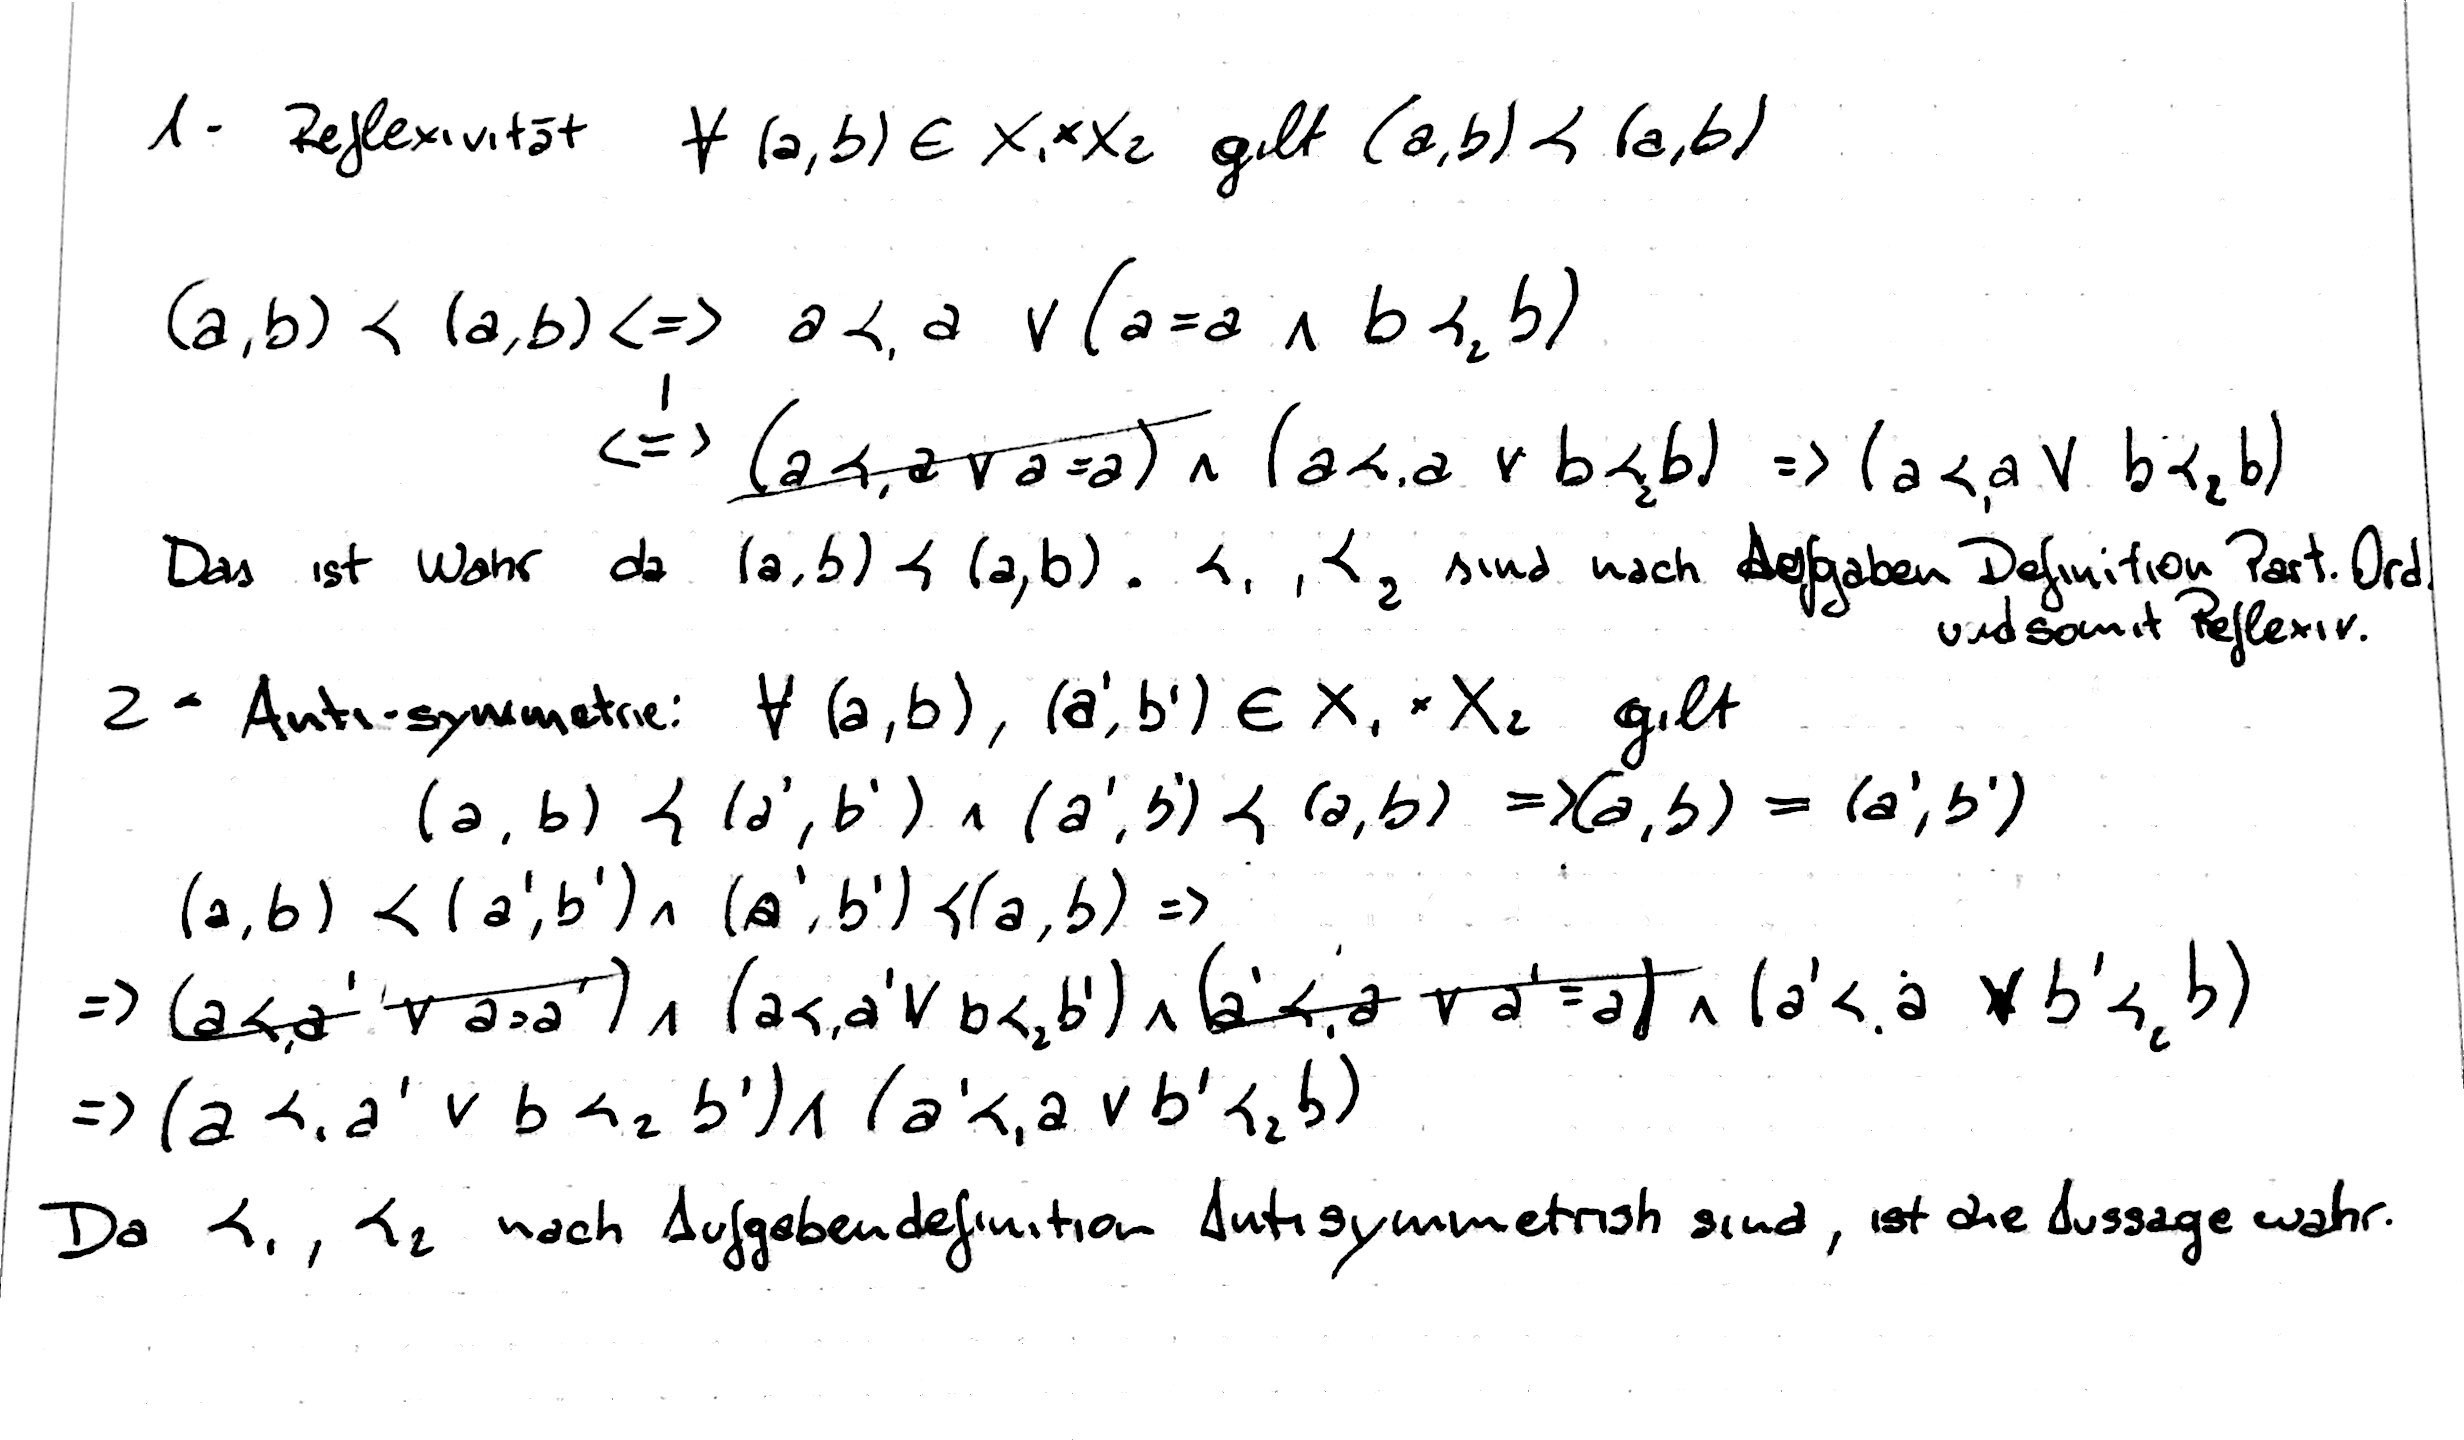
\includegraphics[scale=0.3]{AB2-1a_1.jpg} \newpage
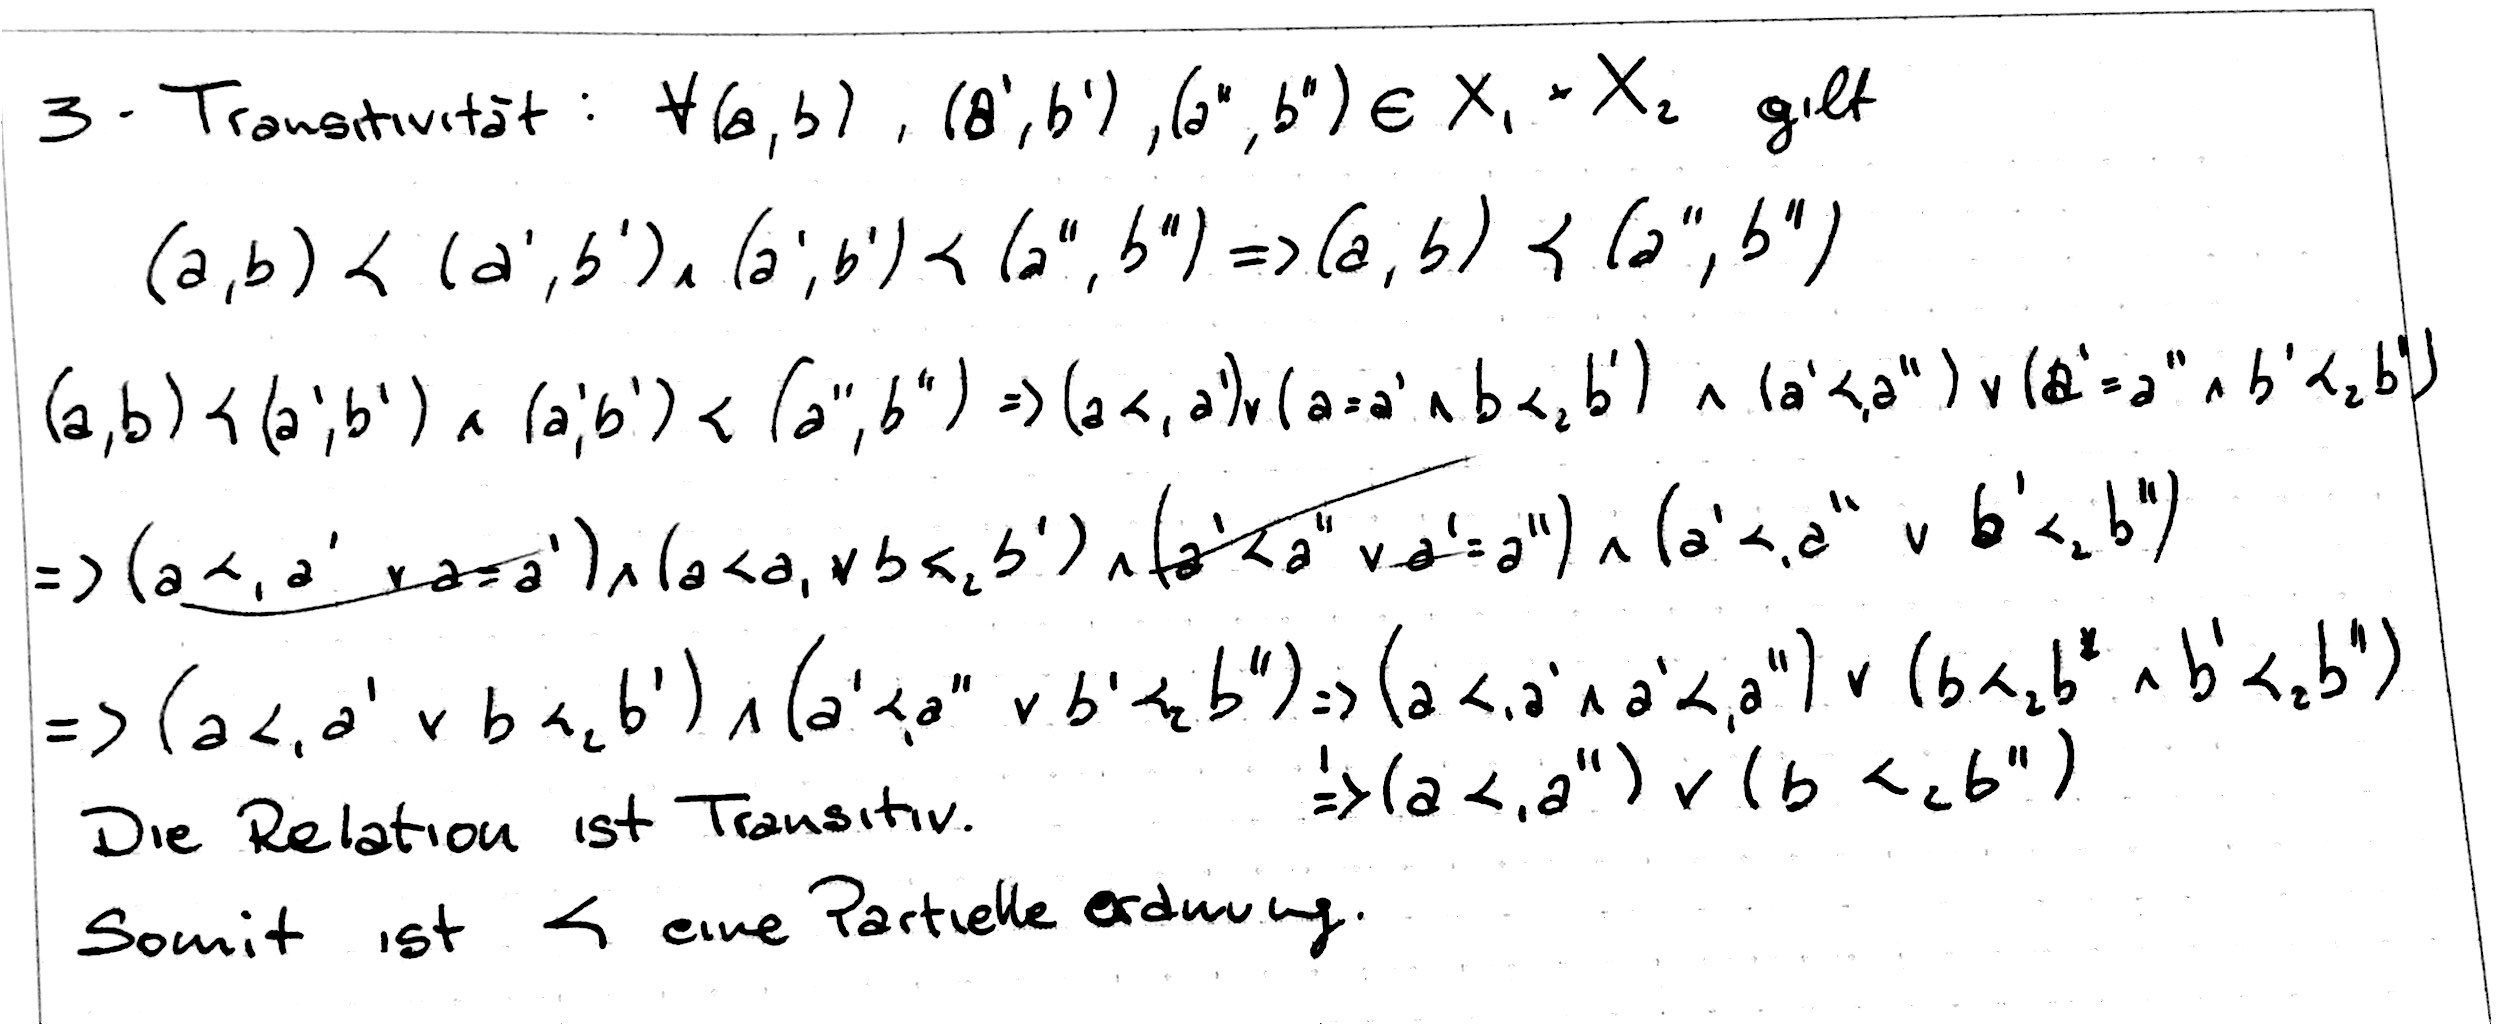
\includegraphics[scale=0.3]{AB2-1a_2.jpg} 
\subsection*{b)}
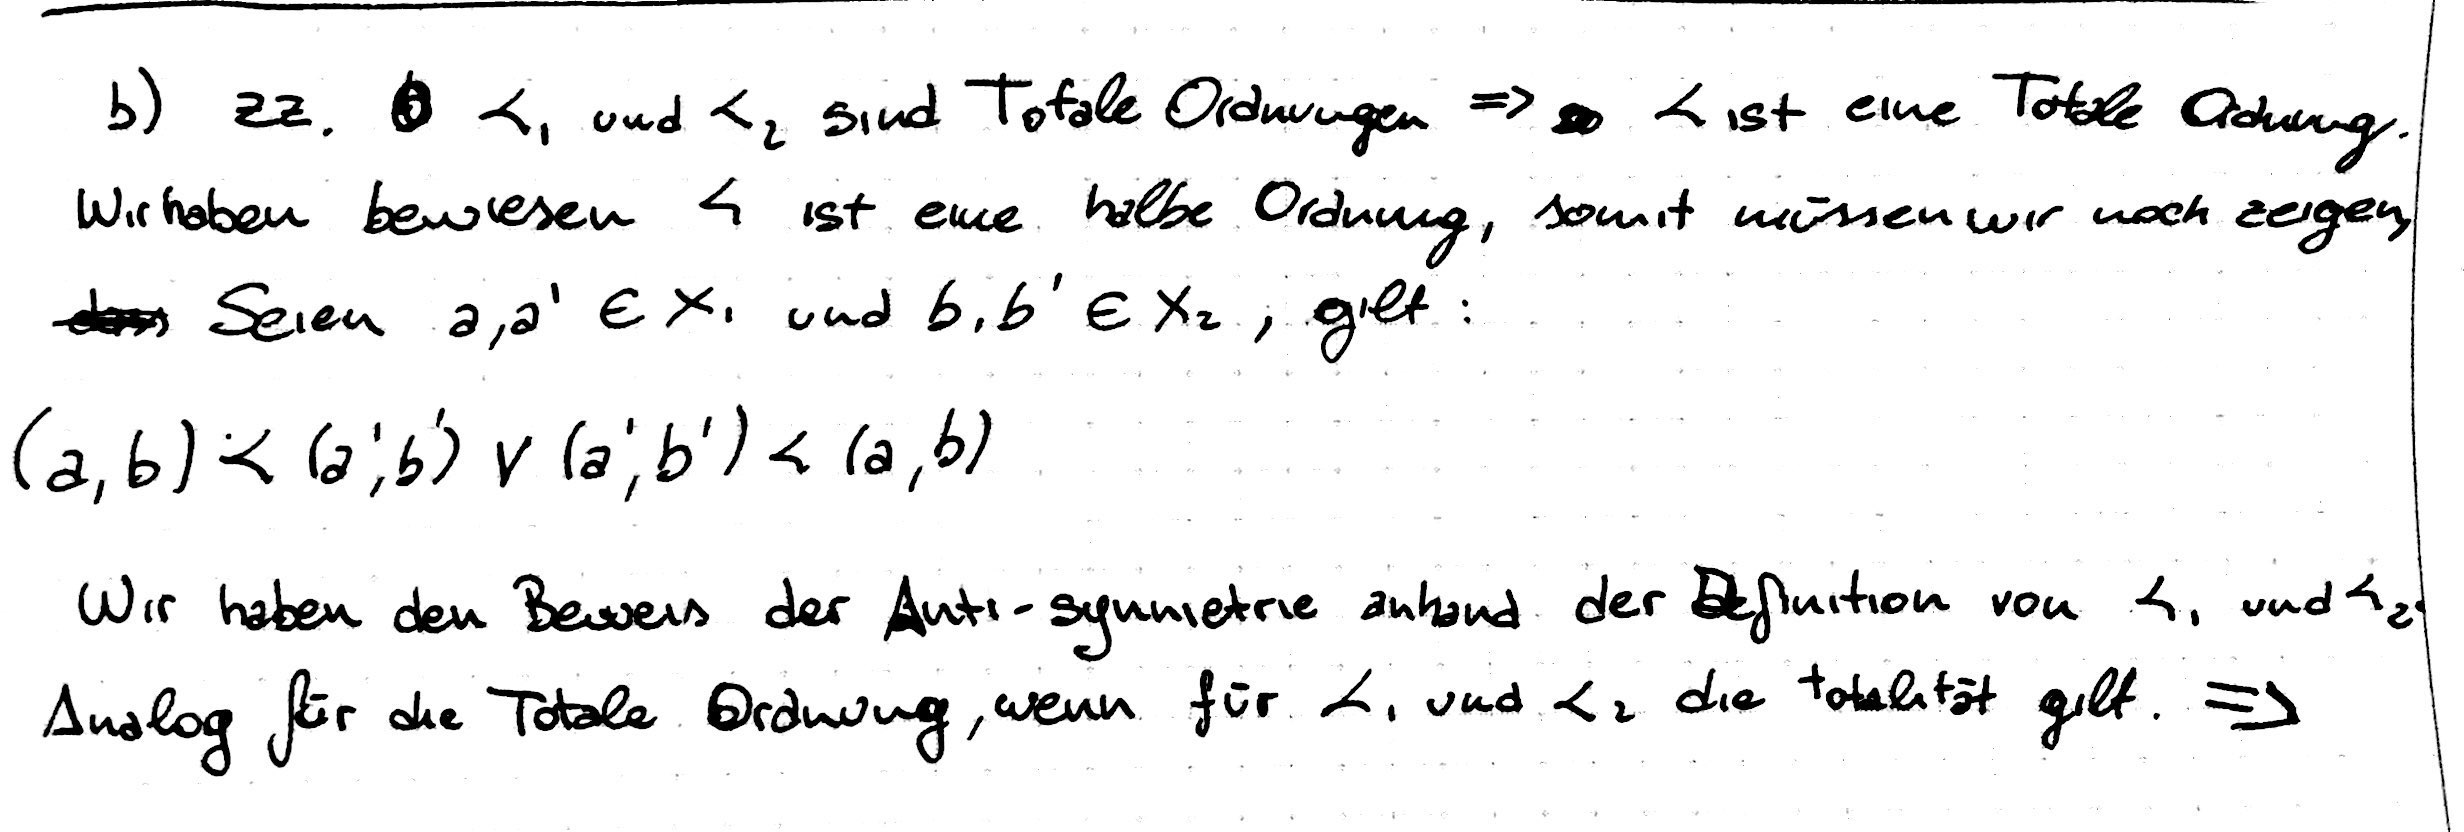
\includegraphics[scale=0.3]{AB2-1b_1.jpg} \\
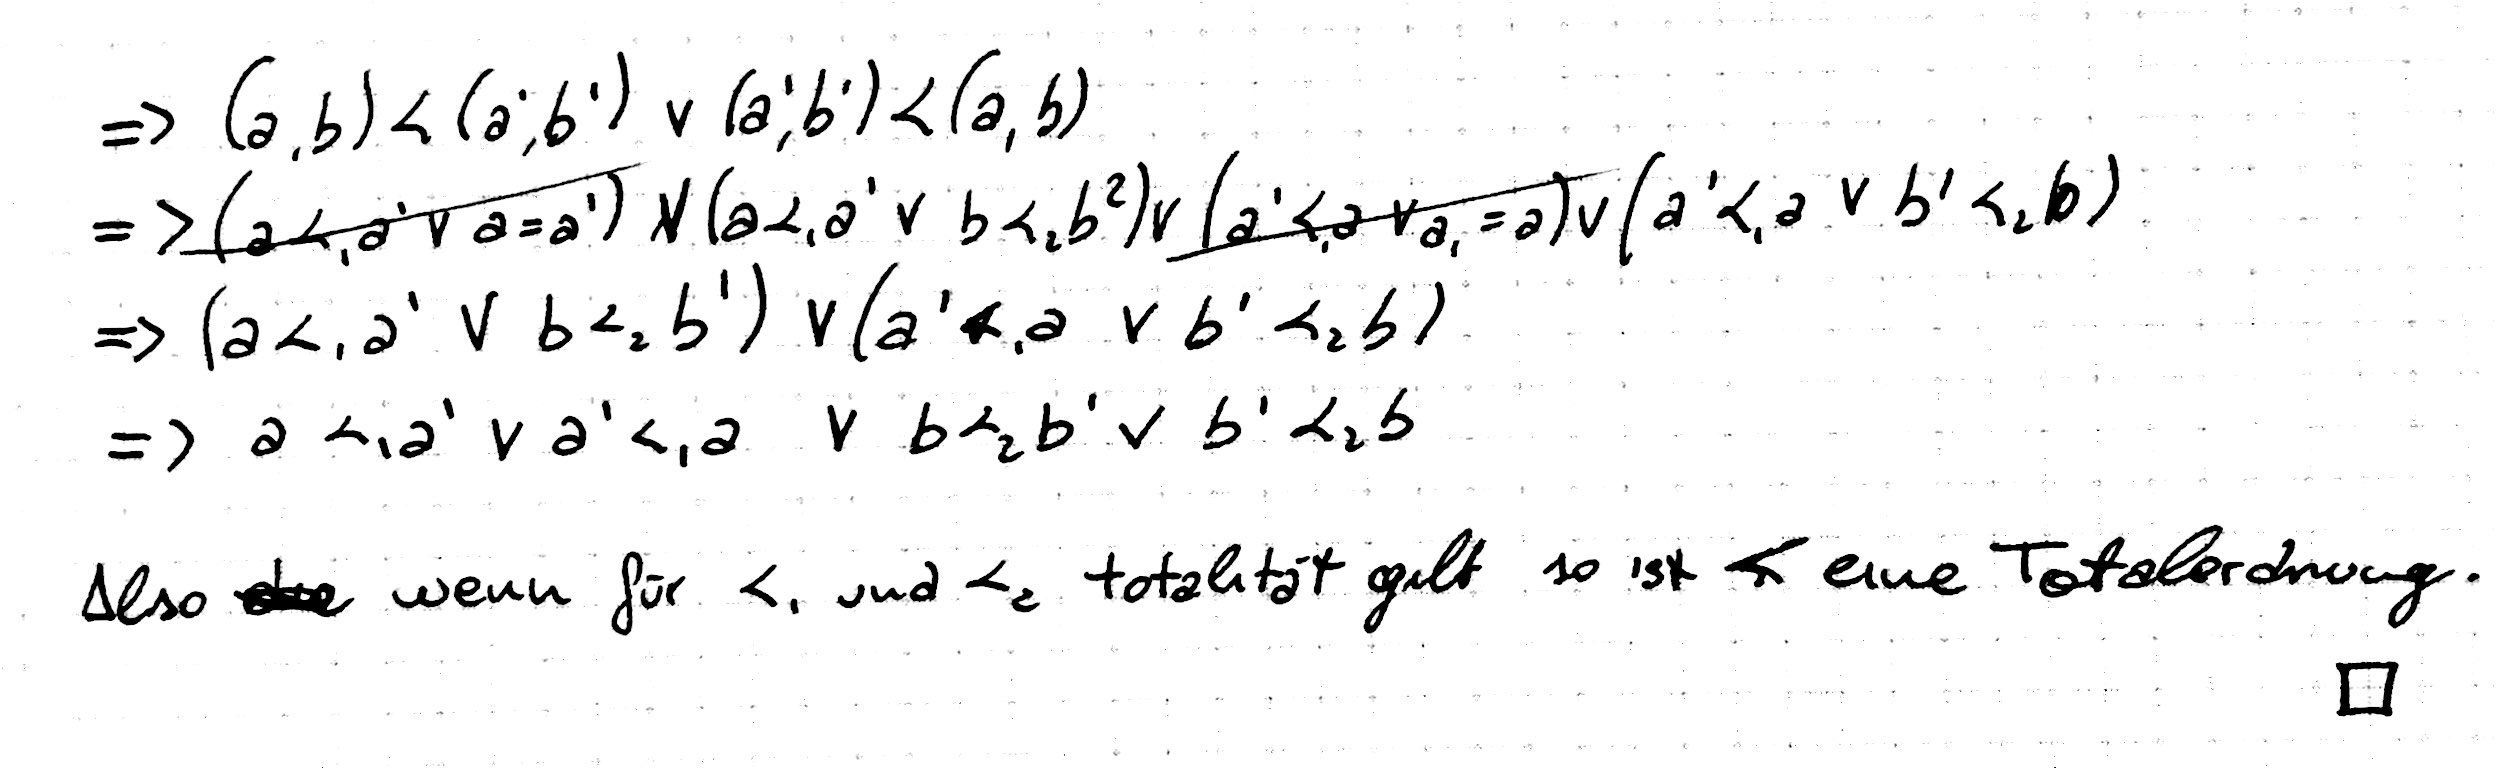
\includegraphics[scale=0.3]{AB2-1b_2.jpg} 
\section*{Aufgabe 2}
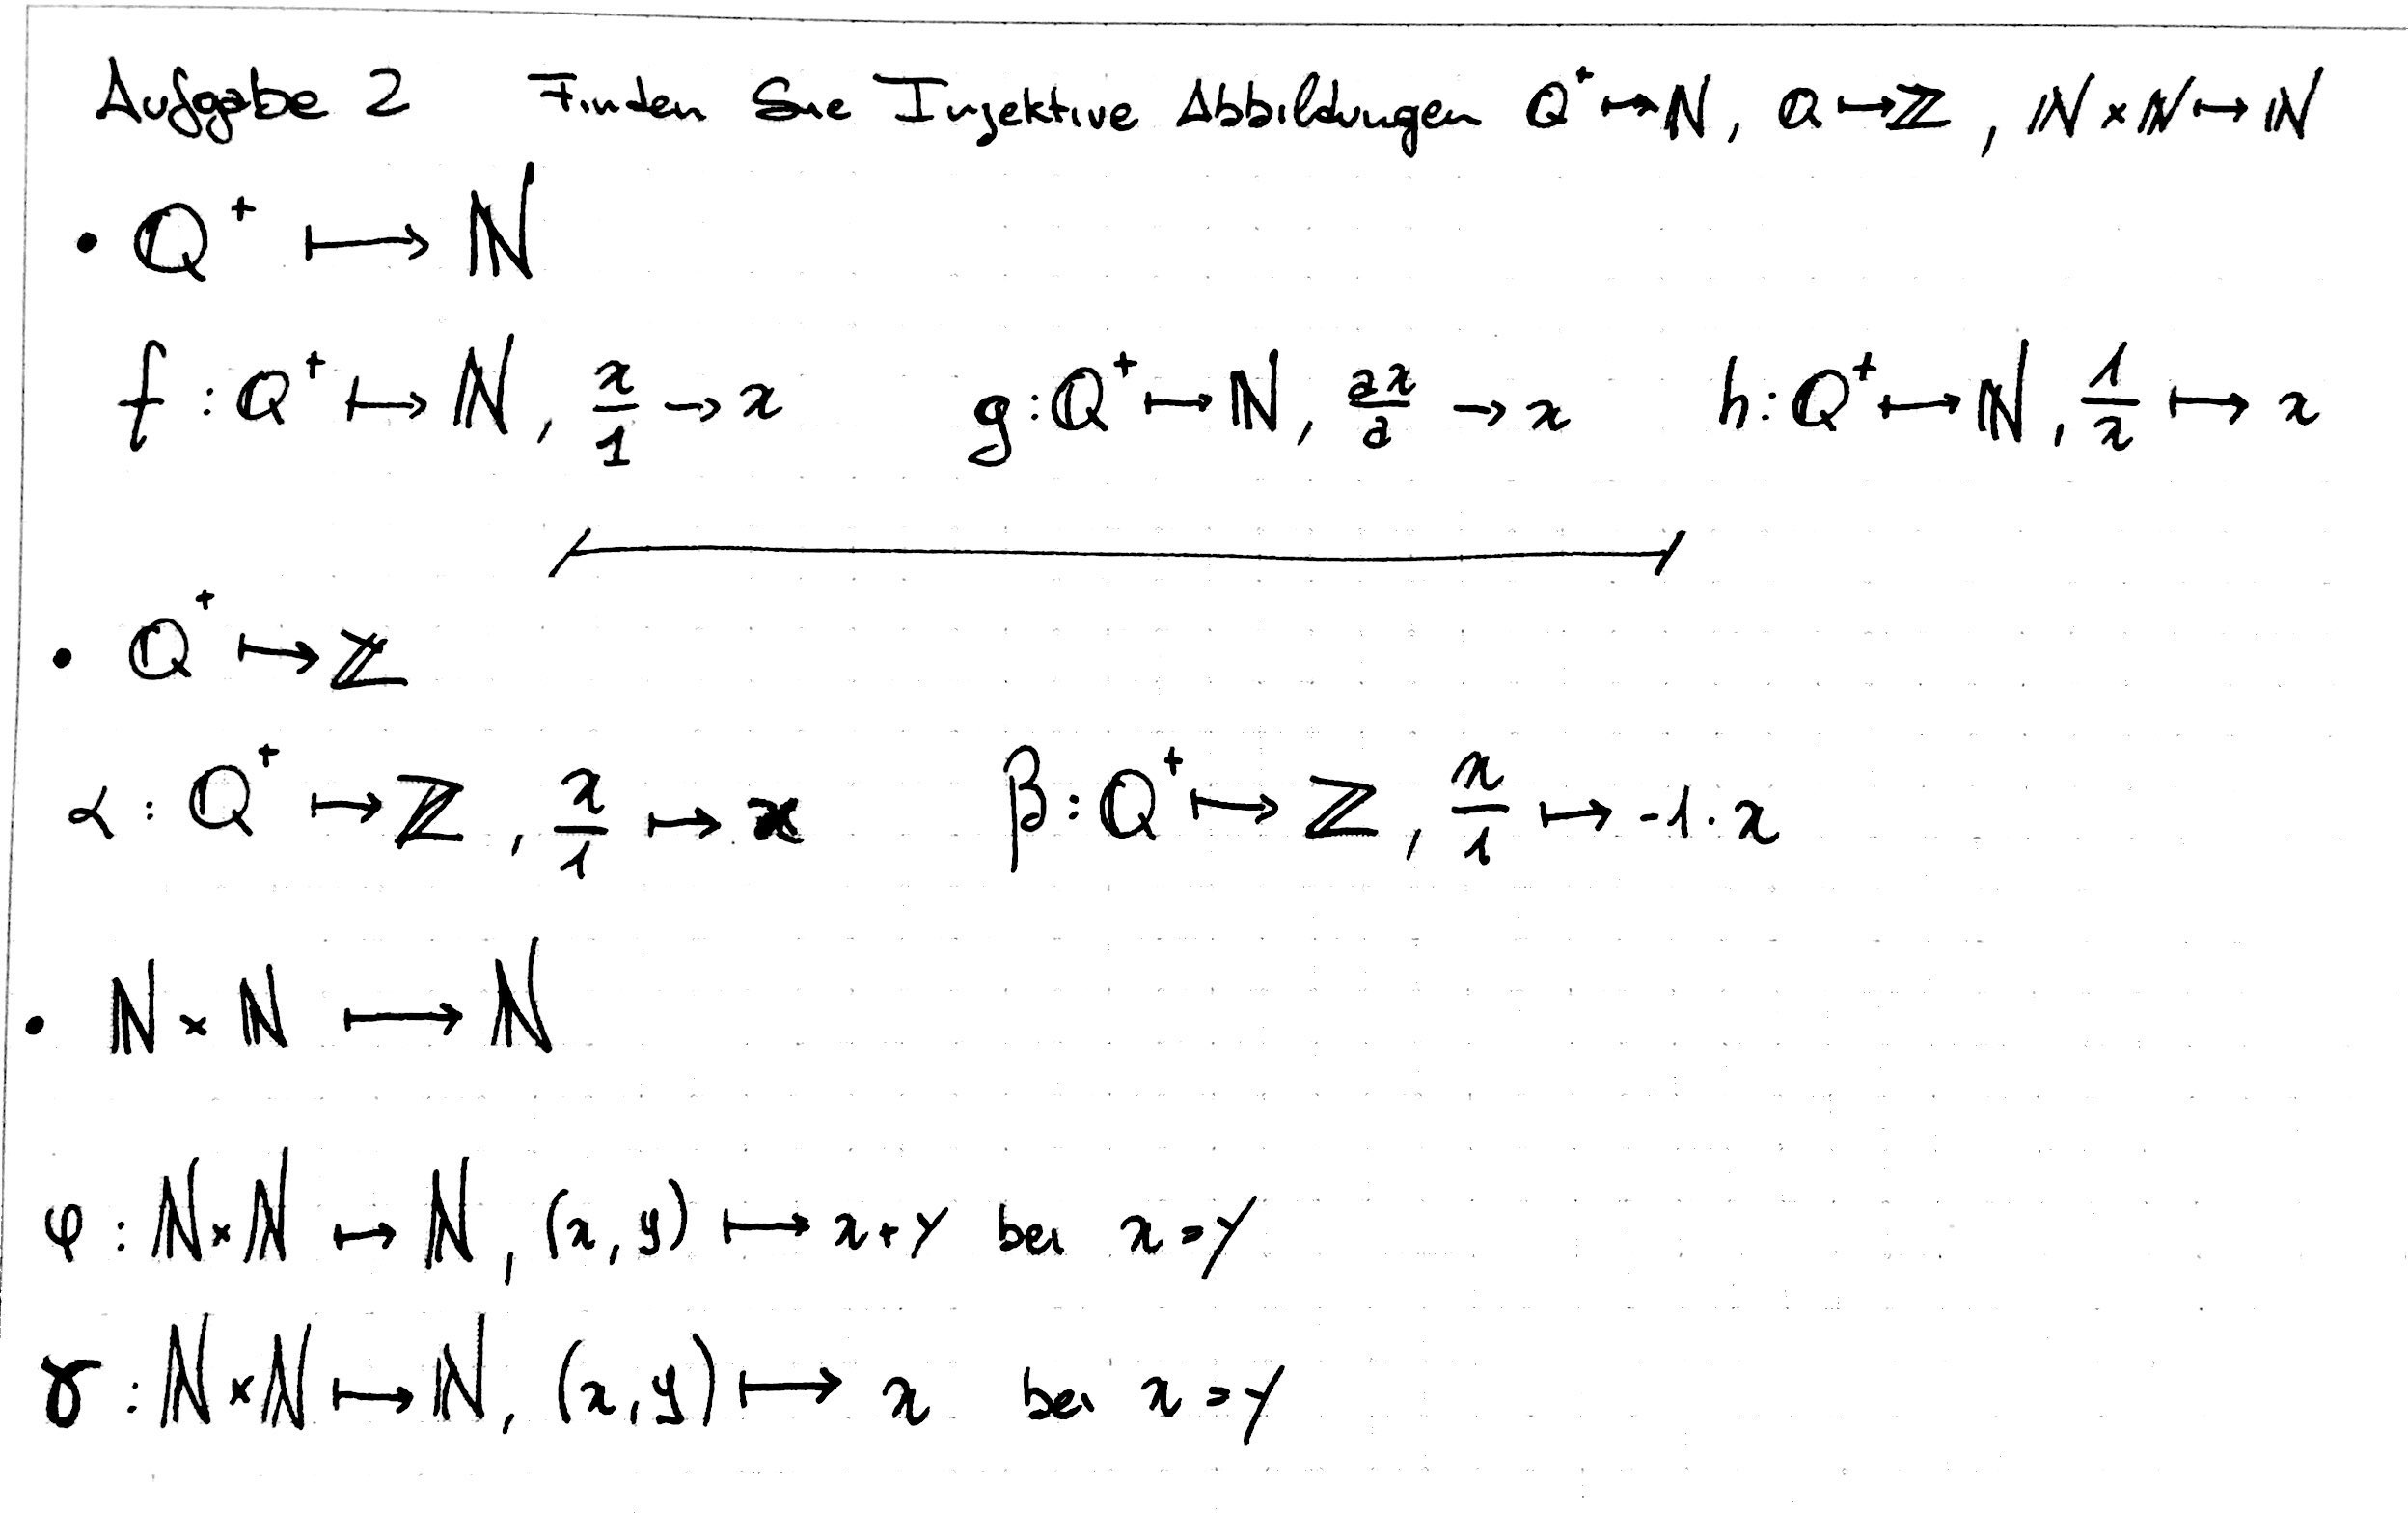
\includegraphics[scale=0.3]{AB2-2_1.jpg} 
\section*{Aufgabe 3}
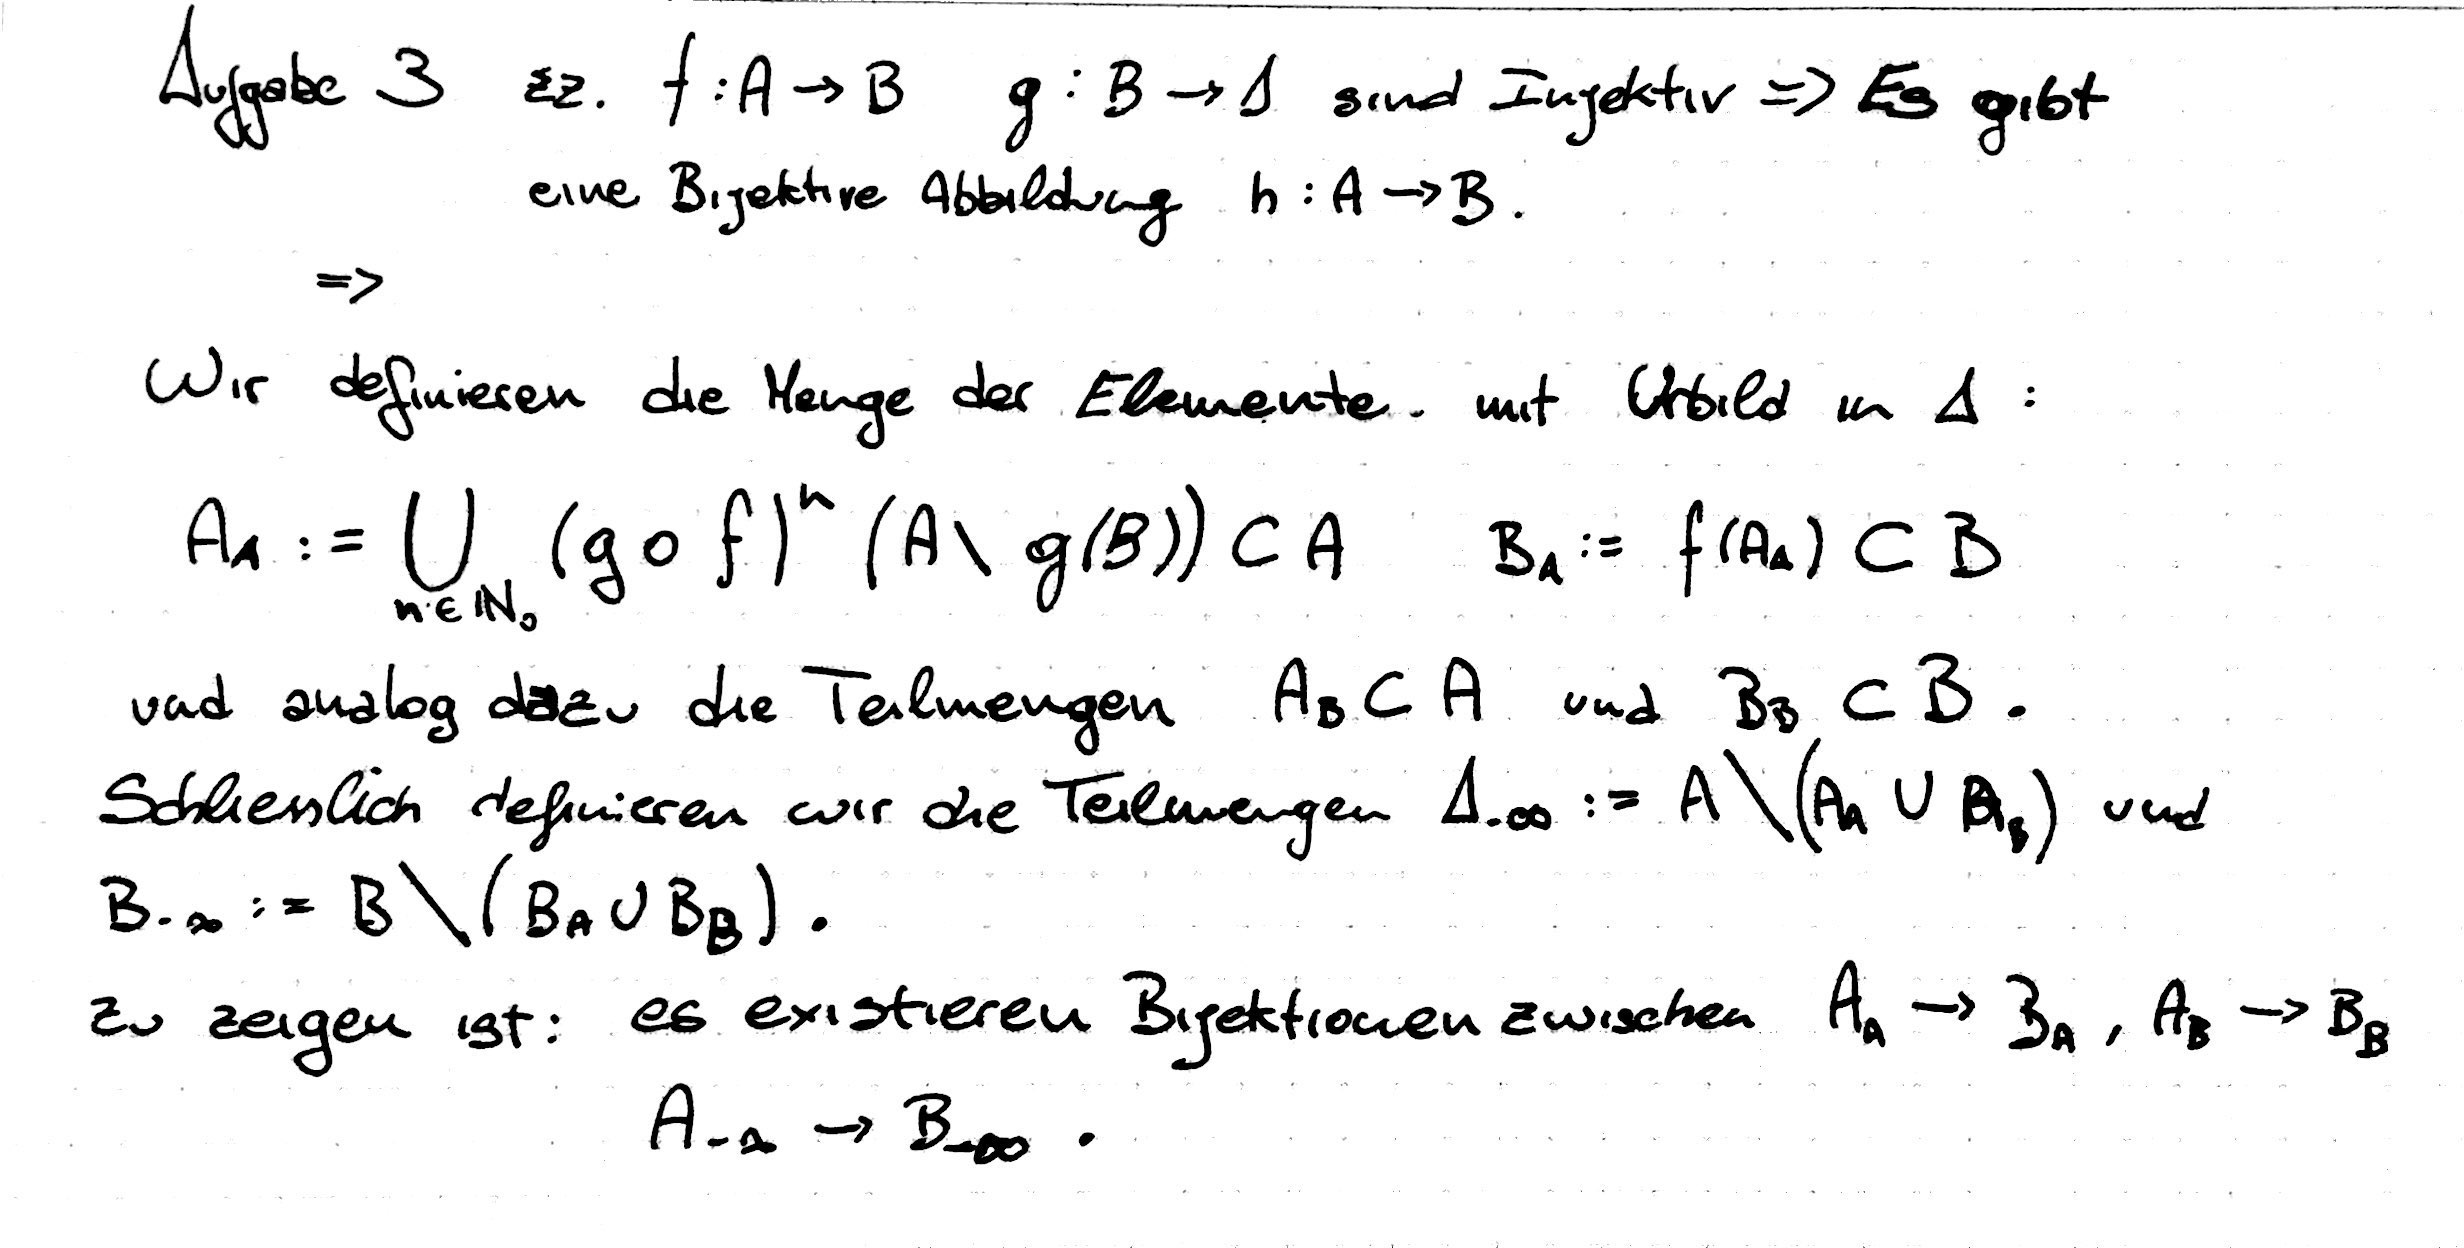
\includegraphics[scale=0.3]{Ab2-3_1.jpg} \newpage
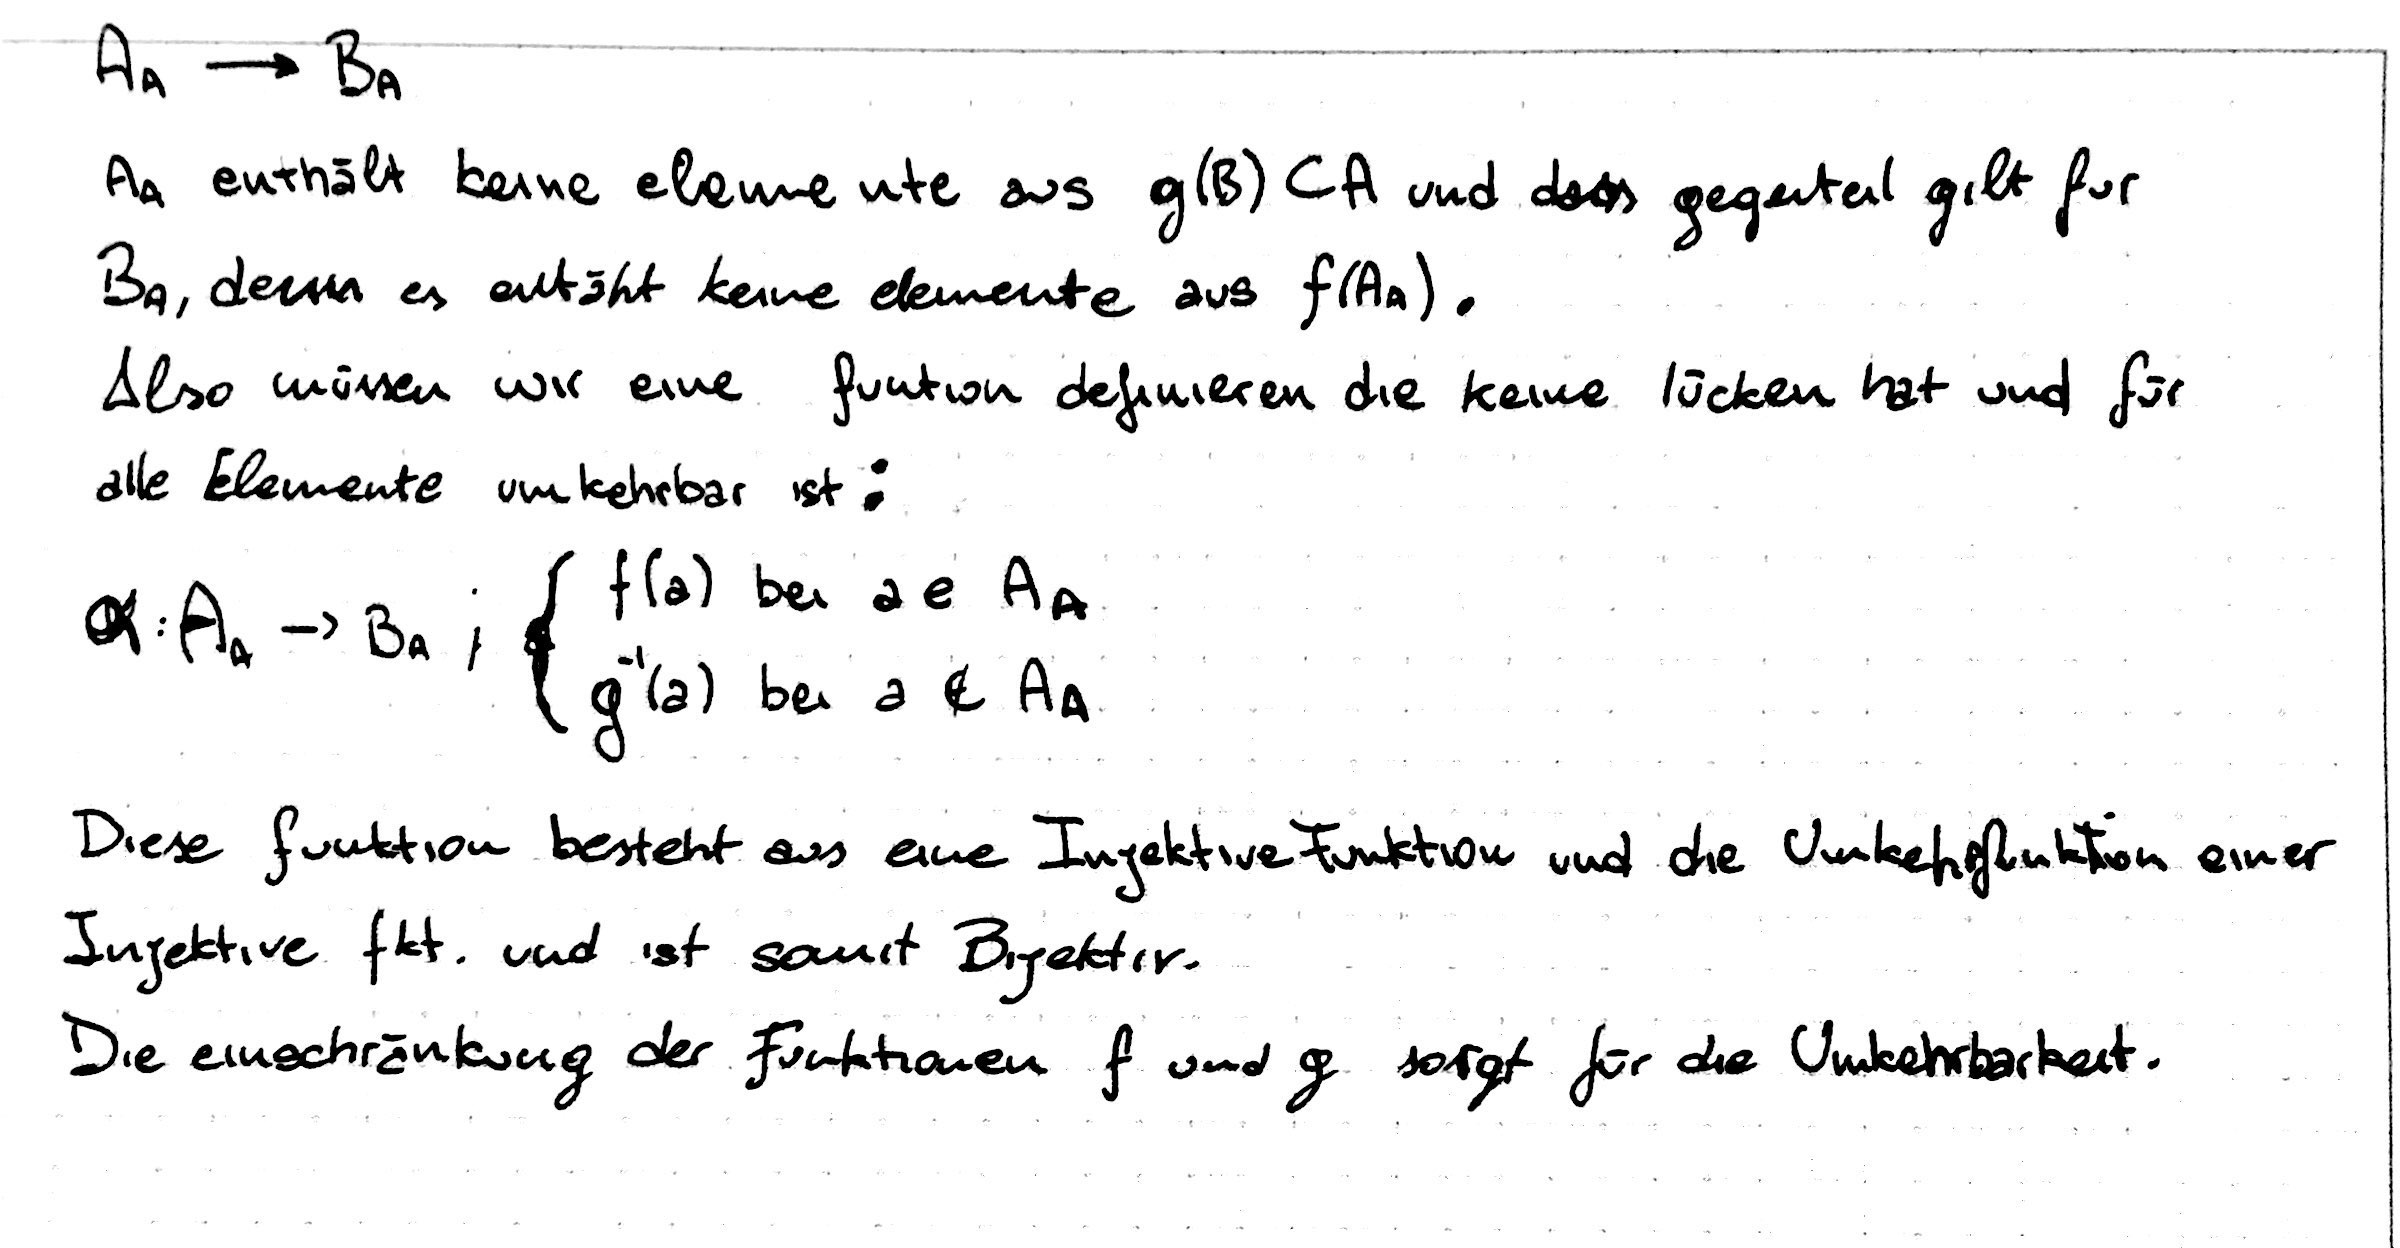
\includegraphics[scale=0.3]{Ab2-3_2.jpg} \newpage
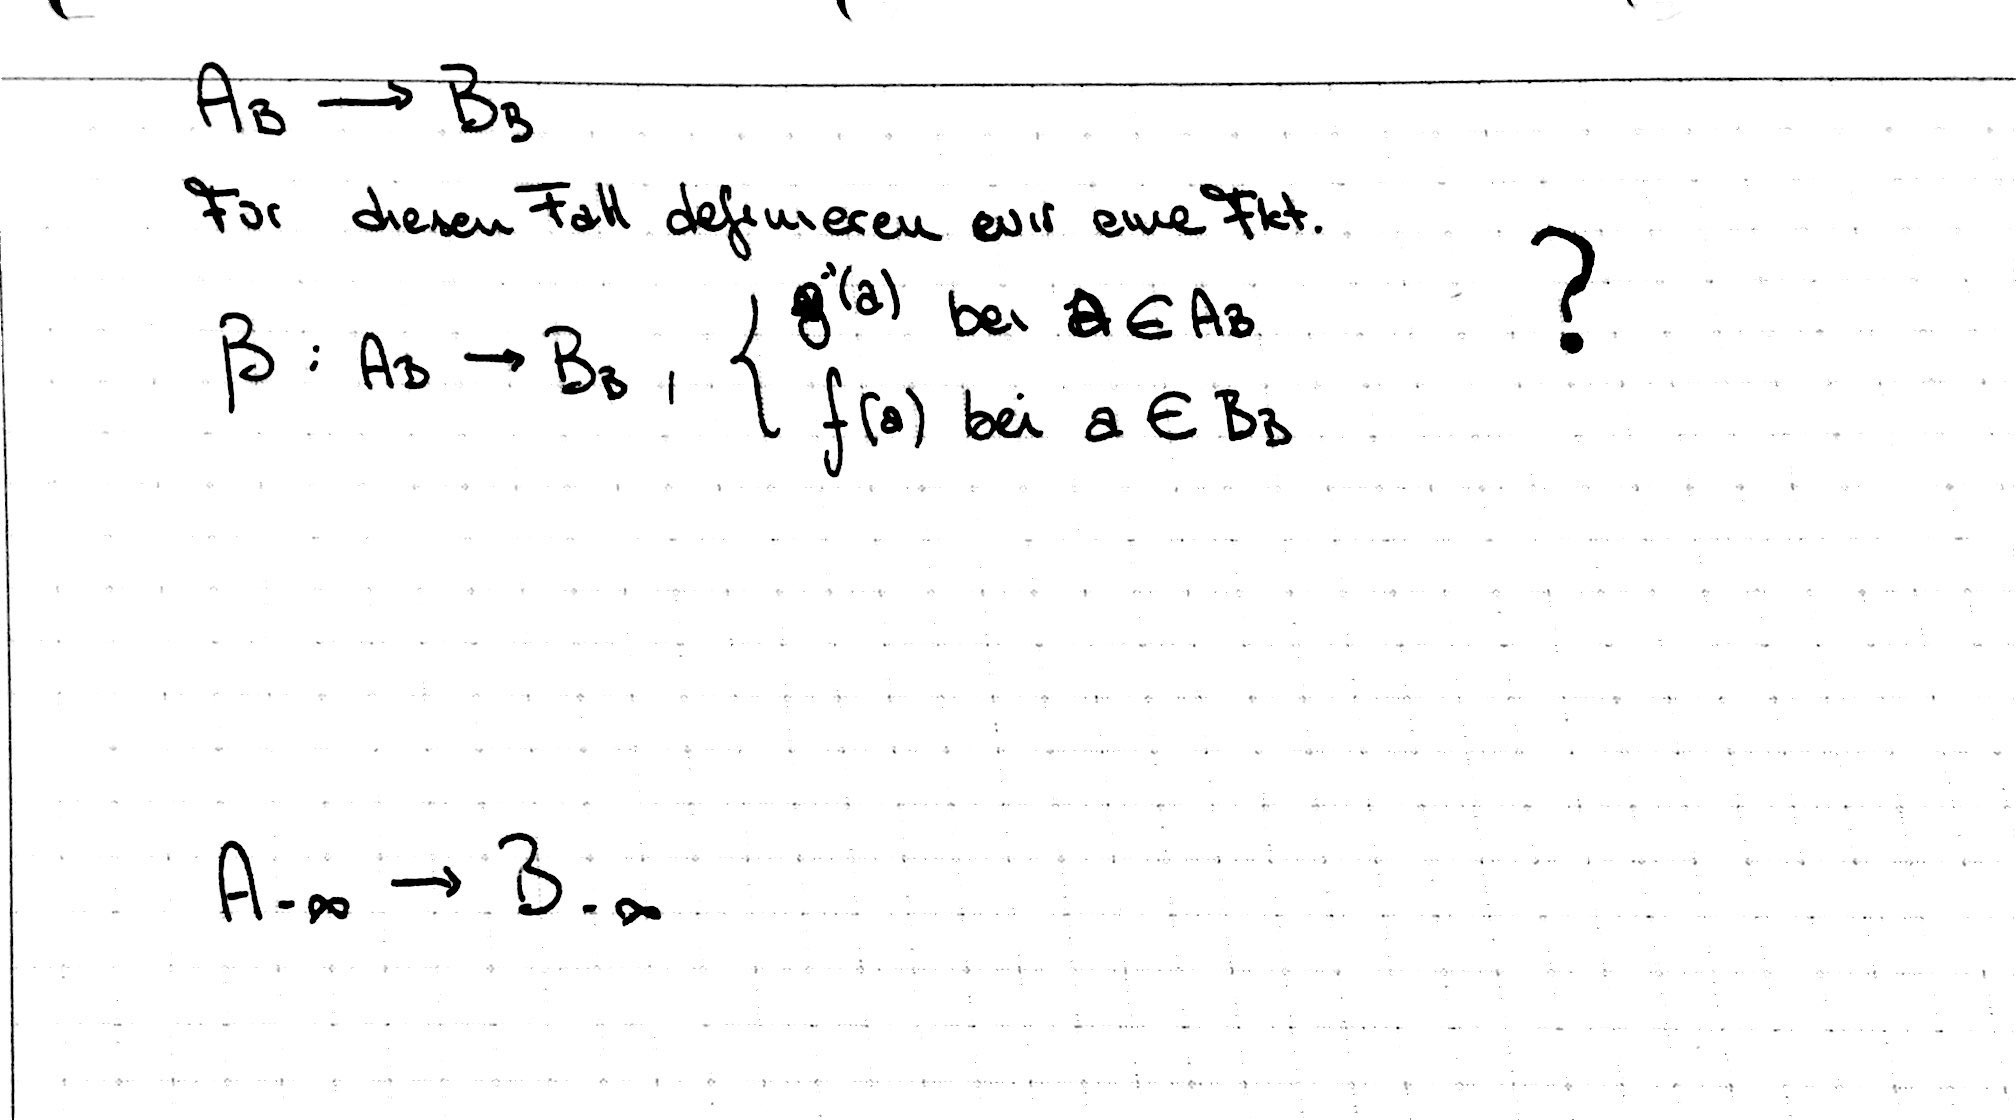
\includegraphics[scale=0.3]{Ab2-3_3.jpg} 
\section*{Aufgabe 4}
\subsection*{a)}
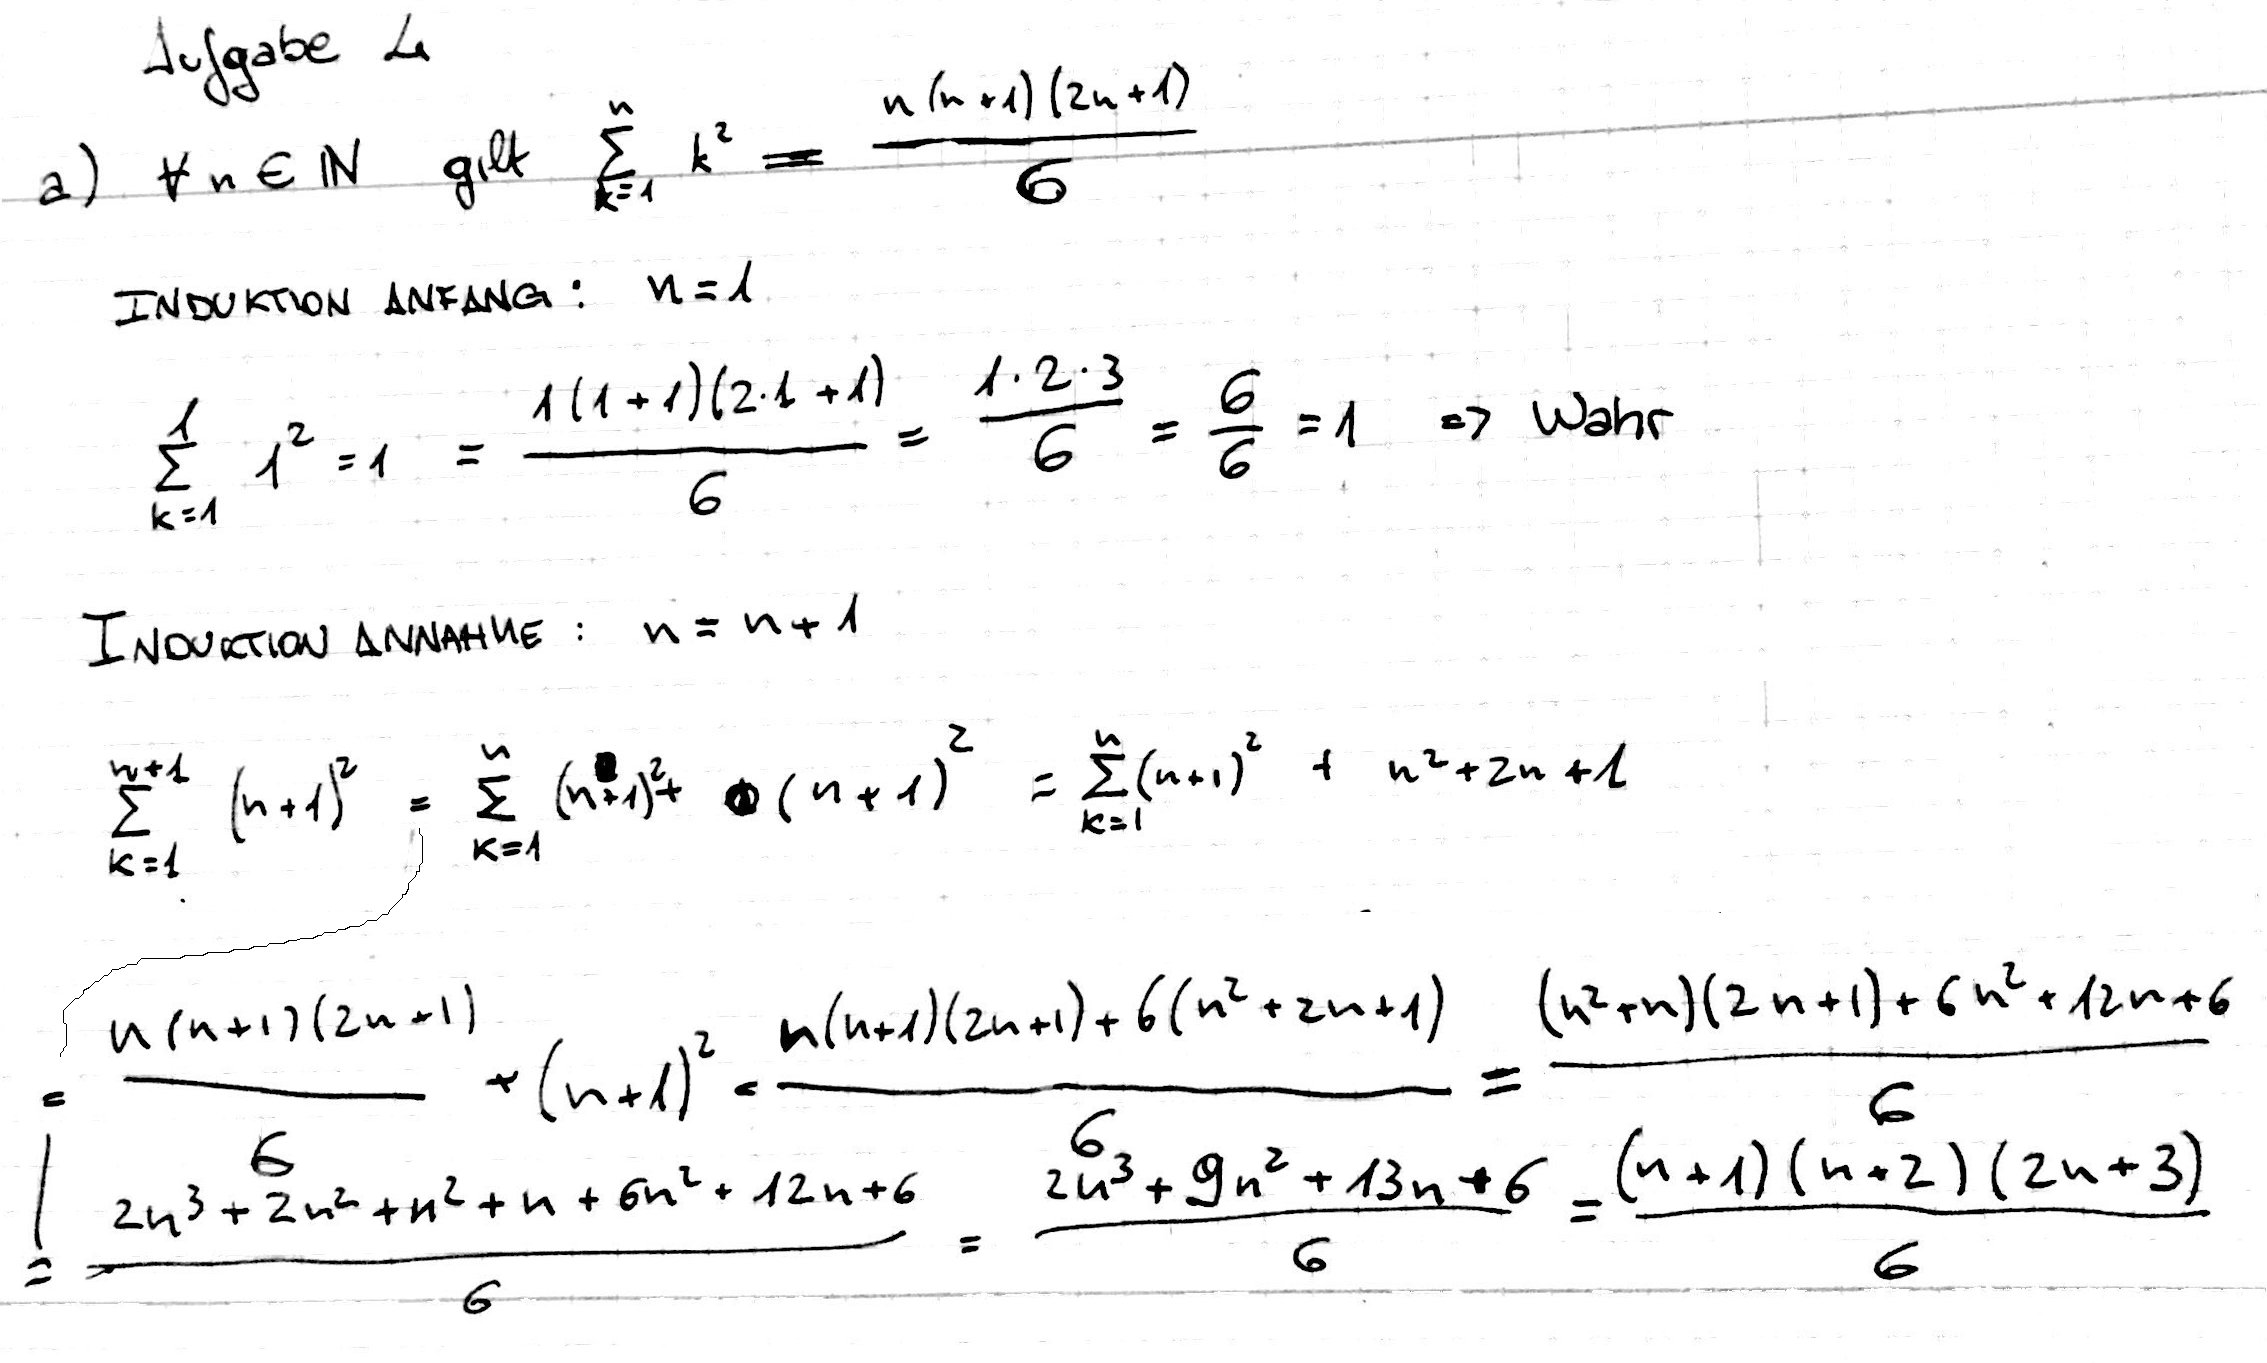
\includegraphics[scale=0.3]{AB2-4_1.jpg} 
\subsection*{b)} 
Bei $k \in \mathbb{N} $ gilt:\\
$
\sum_{k=0}^{n}k^3 = \left( \frac{n \cdot (n+1)}{2} \right)^2
$

\end{document}